\documentclass[11pt]{article}

\usepackage[margin=1in]{geometry}
\usepackage[T1]{fontenc}
\usepackage{lmodern}
\usepackage{amsmath}
\usepackage{booktabs}
\usepackage{graphicx}
\usepackage{caption}
\usepackage{array}
\usepackage{longtable}
\usepackage[round,authoryear]{natbib}
\usepackage[hidelinks]{hyperref}
\usepackage{xurl}

\captionsetup{font=small,labelfont=bf}
\setlength{\parskip}{0.4em}
\setlength{\parindent}{0pt}
\renewcommand{\arraystretch}{1.12}

\newcommand{\HEcov}{\mathrm{HE}_{\mathrm{cover}}}
\newcommand{\HElad}{\mathrm{HE}_{\mathrm{ladder}}}
\newcommand{\dHE}{\Delta\mathrm{HE}}
\newcommand{\degF}{\ensuremath{^\circ}F}

\title{Can Exchange-Traded Weather Contracts Hedge Parametric Cover for Small Businesses?\\[0.3em]
\large Pre-Registered Evidence from Kalshi Station Ladders}

\author{Ehfaz Zoha\\
Princeton University\\

\date{Working paper, draft of September 2026}

\begin{document}
\maketitle

\begin{abstract}
\noindent
Parametric weather cover pays a fixed amount when a weather index crosses a trigger, so it can pay a small business quickly and without a claims process. Its weak point is basis risk: the index is measured at an official station, not at the shop. I ask whether Kalshi's exchange-listed daily weather contracts, which settle on the same official stations, can carry the hedge for such cover, and whether a small extra ``residual'' index can close the gap between the station and a nearby business. Every test was written down and time-stamped before any number was produced. At the settlement station the contracts fit the loss well: a ladder of Kalshi daily-high contracts tracks a capped heat cover with hedge effectiveness (HE) of 0.95 over 4,462 city-days in New York, Chicago and Miami. Price is the problem. Bought 24 hours ahead, the ladder cost 24.6\% more than it paid out, against a pre-registered limit of 20\%, so the main test failed; after paying that price the buyer was worse off than with no hedge (HE $-0.32$). Away from the station, the station leg alone keeps a median HE of 0.81 for heat but only 0.49 for weekly rain at airport stations within 50 km. A residual index built from PRISM grid cells raised the median rain HE to 0.81 (median gain $+0.229$, 95\% CI 0.119 to 0.318), with a gain at 25 of 26 station pairs. No residual design cleared the bar for temperature. Most pre-registered tests in the wider project failed, including every test of whether a business's own weather sensitivity can be learned from public stand-in sales data. I report all of them.
\end{abstract}

\textbf{Keywords:} parametric insurance, basis risk, weather derivatives, prediction markets, hedge effectiveness, pre-registration

\textbf{JEL codes:} G22, G13, Q54

\section{Introduction}

A café loses sales on very hot afternoons. A landscaping crew loses billable days when it rains. Standard business insurance does not pay for either, because nothing was damaged. Parametric (index) cover can: it pays a set amount per degree above a strike, or per inch of rain, read from a published weather record. There is no adjuster and no proof of loss, so a payout can arrive within days.

The catch is basis risk. The cover pays on the index, and the index is measured somewhere else. A heat cover settled at Central Park pays on Central Park's high, not on the temperature outside a café in Queens. If the two disagree, the business can have a bad day and get nothing, or get paid on a day it did fine. A second problem is who carries the risk. A small policy is too small for a reinsurer to price one at a time.

Prediction-market exchanges now list daily weather contracts that could help with both problems. Kalshi, a US exchange regulated by the Commodity Futures Trading Commission, lists daily ``highest temperature'' contracts for several cities. Each day's set of contracts is a ladder of brackets, mostly 2\degF{} wide with open-ended top and bottom brackets, and each bracket pays \$1 if the official high lands in it. The contracts settle on official station readings, and they trade every day. If they are cheap enough, an insurer could write parametric cover for many small businesses and lay off the risk on the exchange. If a small extra contract could cover the gap between the station and the shop, the business would face less basis risk too.

This paper asks whether that works. It reports the evaluation stage of Ceraunic, a prototype design for local weather cover built on Kalshi's station contracts. I split the question into five parts and froze the test rules for each before computing any result:
\begin{enumerate}
\item At the settlement station, does a ladder of Kalshi contracts pay out in line with a parametric heat or rain cover, and at what price (Section~\ref{sec:station})?
\item How much of a nearby business's weather risk does the station leg alone remove (Section~\ref{sec:geo})?
\item Does a residual index contract, settled on gridded or nearby-station data, close the rest of the gap (Section~\ref{sec:residual})?
\item If many businesses buy cover through one pool, how much of the risk cancels, and how much capital must the pool hold (Section~\ref{sec:pool})?
\item Can a business's sensitivity to weather be learned from a year of its own sales (Section~\ref{sec:learn})?
\end{enumerate}

The short answers are mixed, and several are negative. The contracts track the loss closely at the station ($\HEcov = 0.95$). But bought a day ahead, the price already reflects tomorrow's forecast, and over the full history it carried a markup of 24.6\% over payouts. That failed the pre-registered limit of 20\%. A buyer who pays that price keeps very little of the hedge: over all years the result is worse than no hedge at all, and on the cheaper 2025--26 market (a pool I added after seeing the numbers) the buyer keeps $\HElad = 0.37$. For rain, a weekly residual index built from PRISM grid cells passed every pre-registered test and raised the median hedge effectiveness at nearby stations from 0.49 to 0.81. For temperature, no residual design passed. The pool simulations show that netting between businesses is small unless my sector assumptions are right, that the pool's capital looks affordable only if the cover is repriced every day from the forecast, and that a first-loss (junior) layer loses money in a one-in-twenty season under every split I tested. The attempt to learn a business's weather sensitivity from public stand-in data (bikeshare, transit, taxi) failed its main tests.

I think two things make the paper useful even though much of it is negative. First, it separates two hedge-effectiveness numbers that are easy to mix up: whether a contract's payout tracks the loss, and whether a buyer is still better off after paying the contract's price at the time they would actually buy it. Exchange-listed weather contracts score well on the first and badly on the second, because they are priced off the forecast. Second, every rule, threshold and sample was fixed before the results, and every later change is logged with a time stamp. The failures are reported next to the passes.

\section{Related work}
\label{sec:related}

\textbf{Index insurance and basis risk.} Index insurance was developed mainly for farmers in lower-income countries, where loss adjustment is costly \citep{barnett2007}. The main concern in that literature is basis risk. \citet{clarke2016} shows that when basis risk is large, rational demand for index cover can be low or even fall as risk aversion rises, because the policy can fail to pay exactly when it is needed. \citet{jensen2016} measure basis risk directly in a livestock program in Kenya and find it large enough that the cover leaves much of household risk in place. \citet{carter2017} review the evidence and argue that the quality of the index, not just its price, decides whether index insurance helps. My setting is different (urban small businesses, daily indices, liquid exchange contracts), but the question is the same: how much of the real loss does the index pay?

\textbf{Geographic basis and multi-site indices.} \citet{woodard2008} show that hedging a local weather exposure with a contract on a distant station loses much of the hedge, and that combining several stations helps. \citet{norton2013} measure how basis risk grows with distance between weather stations. \citet{ritter2014} model rainfall jointly at several sites to reduce geographic basis risk in rainfall derivatives, and \citet{odening2007} discuss the pitfalls of pricing rainfall derivatives from daily models. My residual designs (Section~\ref{sec:residual}) are a small, pre-registered horse race over this family of ideas: grid cells, regional averages and nearby-station pairs.

\textbf{Weather derivatives.} The pricing literature models temperature as a mean-reverting process and prices degree-day contracts off it \citep{alaton2002,caowei2004,jewson2005}. \citet{campbell2005} show that forecasts matter for pricing: once a good forecast exists, the contract's value moves with it. That is the mechanism behind my main negative result. \citet{golden2007} discuss basis and credit risk in weather hedging, and \citet{perezgonzalez2013} find that firms using weather derivatives are valued more highly. The exchange-traded weather contracts in that literature are mostly monthly or seasonal degree-day futures. Daily station contracts that a small buyer can trade are newer.

\textbf{Prediction markets.} Prices in prediction markets are often read as probabilities \citep{wolfers2004}, though \citet{manski2006} shows that this reading needs assumptions about traders, and \citet{snowberg2010} document a favorite--long shot bias in betting markets. I use Kalshi prices both ways: as a forecast (scored by the Brier score, \citealp{brier1950}) and as a cost of hedging. The hedge-effectiveness measure follows \citet{ederington1979}.

\textbf{Pre-registration.} Pre-registration fixes the analysis before the data are seen, so that the number of tests run and the choices made cannot be tuned to the result \citep{nosek2018}. It is common in experimental work and rarer in empirical finance. I use it here because the project had commercial goals, and a design study run by people who want a product to work is exactly where tuning is most tempting.

\section{Setting}
\label{sec:setting}

\subsection{The cover}

The heat cover in the main tests pays \$1 for each \degF{} by which the official daily high at the settlement station exceeds a strike $K$, capped at 6\degF{}:
\begin{equation}
H(T;K) = \min\bigl(\max(T - K, 0),\, 6\bigr),
\end{equation}
per unit per day, where $T$ is the integer daily high. One ``unit'' therefore pays at most \$6 a day. For the station tests the strike is the lower edge of the ladder's second bracket (``rule A''); Section~\ref{sec:station} also reports a strike fixed in advance from the trailing seven-day mean (``rule B''). For the geography and residual tests the strike is the floor of the trailing seven-day mean at the settlement station, the same for every point that day.

The rain covers are a daily wet-day binary (pays \$1 if the station records at least 0.01 in) and a weekly total (pays \$1 per inch of Monday--Sunday rainfall, capped at 3 in).

\subsection{The hedge}

A Kalshi daily-high ladder for a city-day is a set of brackets, each a contract paying \$1 if the settled high lands in it. Buying $H(v_b;K)$ contracts of each bracket $b$, where $v_b$ is a representative value inside the bracket, replicates the cover up to the 2\degF{} bracket width. Prices are the YES ask from Kalshi's hourly candles, taken at 24, 12 or 2 hours before the market closes, with Kalshi's taker fee added (0.07 $\times$ contracts $\times$ $P(1-P)$ per order, rounded up to the cent; I could not fetch Kalshi's fee schedule, so this formula is medium confidence).

\subsection{Two hedge-effectiveness numbers}

Let $E$ be the cover's payout (the business's exposure), $X$ the ladder's payout, and $\pi$ the premium plus fees paid at the decision time. I report
\begin{align}
\HEcov &= 1 - \frac{\operatorname{Var}(E - X)}{\operatorname{Var}(E)}, \\
\HElad &= 1 - \frac{\operatorname{Var}\bigl(E - (X - \pi)\bigr)}{\operatorname{Var}(E)}.
\end{align}
$\HEcov$ asks whether the contract's payout tracks the loss. $\HElad$ asks whether a buyer who pays the market price at the time they would really buy is steadier than one who does nothing. A value of 1 removes all variance, 0 removes none, and a negative value adds variance. The two differ because the price $\pi$ moves with the forecast: a buyer one day ahead swaps the weather swing for a price swing of nearly the same size, and keeps only the forecast miss.

\subsection{Two legs: station plus residual}

For a business near but not at the settlement station, I split the hedge into two legs. The \emph{station leg} pays on the station, where a Kalshi ladder exists. The \emph{residual leg} $r$ is a separate index contract, settled on published data, that pays the estimated difference between the business's location and the station. The business holds both, and the test is how much the residual adds:
\begin{equation}
\mathrm{HE} = 1 - \frac{\operatorname{Var}(E_b - H_S - r_b)}{\operatorname{Var}(E_b)}, \qquad \dHE = \mathrm{HE} - \mathrm{HE}(\text{station leg alone}).
\end{equation}
There is no exchange market for residual contracts. In the design, a capitalised pool would write them. Section~\ref{sec:pool} asks what that pool would need to hold.

\section{Data}
\label{sec:data}

All data are free and were pulled without accounts or keys. Nothing was traded.

\begin{itemize}
\item \textbf{Kalshi markets and hourly candles}: 61 weather series in five cities, 34,495 markets and 1,113,358 hourly candle rows. The station tests use every settled daily-high ladder for New York (Central Park, from 2022-04-27), Chicago (Midway, same span) and Miami (from 2023-05-11), through 2026-09-28; thin ladders for Newark (EWR) and Trenton (TTN) from 2026-08-26; and 1,053 daily rain binaries.
\item \textbf{Order books}: Kalshi keeps no book archive, and the recorder I planned to use was not readable when the tests ran. Depth comes from one snapshot taken on 2026-09-29.
\item \textbf{Official station records}: the National Weather Service daily climate reports (6,832 rows from 2023 onward, plus an archive of 10,054 issued reports to measure revisions), Iowa Environmental Mesonet ASOS daily summaries for 26 stations, and GHCN-Daily station histories back to the 1950s \citep{menne2012}.
\item \textbf{Gridded data}: PRISM 4 km daily grids \citep{daly2008} and NOAA nClimGrid-Daily \citep{durre2022}, including 50 preliminary vintages of nClimGrid to measure revisions.
\item \textbf{Business population}: Census ZIP Business Patterns 2023 and SUSB 2022 (1,109,492 small establishments in the sectors used).
\item \textbf{Sales stand-ins} (Section~\ref{sec:learn}): daily Citi Bike, Divvy, Chicago CTA rail, Chicago taxi and New York TLC taxi data from 2022-07-01.
\end{itemize}

Two conventions matter for reading the numbers. The join key is the NWS climate day (midnight to midnight local standard time), and every decision time is computed from each market's own close time, so no price uses information from after the decision. A gridded file labelled day $D$ describes calendar day $D-1$, and the code aligns them that way.

\section{Pre-registered design}
\label{sec:prereg}

The work ran in phases. Before each phase produced a number, its sample, method and pass/fail thresholds were written into a pre-registration file and time-stamped in UTC. Table~\ref{tab:tests} lists the main tests. Point estimates decide pass or fail; confidence intervals are reported alongside. Intervals are 95\% block-bootstrap percentile intervals \citep{kunsch1989,politis1992}: 7-day calendar blocks for the station tests, a joint circular bootstrap with 14-day blocks (2-week blocks for weekly rain), 2,000 draws and the same resampled calendar for every location for the residual tests. Every change after a freeze is logged with its time and whether it came before or after the first result (Section~\ref{sec:failures} and Appendix~\ref{app:ledger}).

\begin{table}[ht]
\centering
\small
\caption{Main pre-registered tests and verdicts. Full ledger in Appendix~\ref{app:ledger}.}
\label{tab:tests}
\setlength{\tabcolsep}{4pt}
\begin{tabular}{p{2.0cm}p{5.9cm}p{3.4cm}l}
\toprule
Test & Rule (frozen before results) & Result & Verdict \\
\midrule
Station T1 & Liquid ladders, 24 h, pooled: $\HEcov \ge 0.85$ and markup $\le 20\%$ & $\HEcov$ 0.95; markup 24.6\% & FAIL \\
Station T2 & Thin ladders (EWR, TTN) fail if 24 h markup $> 100\%$ & 241\%, 266\% & FAIL \\
Station T3 & Rain binary: Brier gain over climatology $\ge 0.02$ at 24 h & 0.141 & PASS \\
Station T4 & No-offer share $\le 10\%$ in every city-year from 2024 & worst 13.7\% (MIA 2024) & FAIL \\
Residual, heat & A design survives only if P1--P4 all pass (below) & best $\dHE$ $+0.061$ & FAIL (none) \\
Residual, rain & Same rules, weekly totals & G1-P $\dHE$ $+0.229$ & PASS (G1-P) \\
Pool M1 & Netting $\ge 0.25$ at $\ge 3$ of 5 stations & 3 of 5 & PASS (minimum) \\
Pool M3 & 30-day capital / pool notional $\le 0.35$ & 0.126 & PASS \\
Pool M5 & VaR backtest not rejected (Kupiec, 5\%) & 1 breach in 599 days & FAIL (too few) \\
Junior & 1-in-20 junior return positive over 3 seasons & $-190\%$ & FAIL \\
Learning T2 & Learned hedge removes $\ge 0.20$ of sales-surprise variance & 0.072, 0.053 & FAIL \\
\bottomrule
\end{tabular}
\end{table}

The residual rules were: \textbf{P1 (gain)} pooled median $\dHE \ge +0.10$ with the lower confidence bound above zero; \textbf{P2 (breadth)} $\dHE > 0$ at $\ge 70\%$ of station pairs and in at least 4 of 5 markets (3 of 5 for rain); \textbf{P3 (efficiency)} pooled median $\eta \ge 0.5$, where $\eta = 2\beta - 1$ and $\beta$ is the regression slope of the unhedged basis on the residual, so that $\eta$ measures how much of the variance the residual hands to the pool actually removes risk from the business; and \textbf{P4 (settleable)} a fixed written formula on published data, a first settlement value within 7 days and a stated revision policy. A design whose pooled median $\dHE \le 0$ is dropped.

\section{Results}

\subsection{At the station: the payout fits, the price does not}
\label{sec:station}

Table~\ref{tab:station} shows the main station result. Across 4,462 city-days in the three liquid cities, the ladder's payout tracks the capped heat cover with $\HEcov = 0.95$ [0.95, 0.96]. The 2\degF{} brackets cost little: the binning error has a root mean square of 0.42 per unit. The settled value matched the NWS climate report on all but 0.2\% of 3,822 city-days since 2023.

\begin{table}[ht]
\centering
\small
\caption{Kalshi heat ladder as a hedge for the capped heat cover, 24 h before close, strike rule A. Premium and payout per \$1/\degF{} unit per day; markup (overround) = premium / payout $-$ 1, fees excluded. 95\% block-bootstrap intervals in brackets. The 2025+ row was added after the results and is not a verdict.}
\label{tab:station}
\footnotesize
\setlength{\tabcolsep}{4pt}
\begin{tabular}{lrrrrrr}
\toprule
Ladder & City-days & Premium & Payout & Markup & $\HEcov$ & $\HElad$ \\
\midrule
Liquid NY+CHI+MIA & 4,462 & 4.73 & 3.79 & 24.6\% [21.4, 27.9] & 0.95 & $-0.32$ [$-0.47$, $-0.20$] \\
Liquid, 2025+ (post hoc) & 1,907 & 4.00 & 3.65 & 9.7\% [7.7, 11.7] & 0.96 & 0.37 [0.33, 0.42] \\
New York (Central Park) & 1,612 & 4.07 & 3.11 & 31.0\% & 0.96 & $-0.23$ \\
Chicago (Midway) & 1,615 & 4.56 & 3.66 & 24.7\% & 0.96 & $-0.34$ \\
Miami & 1,235 & 5.80 & 4.88 & 19.0\% & 0.93 & $-0.59$ \\
Newark (thin) & 34 & 8.93 & 2.62 & 241.2\% & 0.95 & $-7.39$ \\
Trenton (thin) & 34 & 8.87 & 2.42 & 265.7\% & 0.90 & $-13.94$ \\
\bottomrule
\end{tabular}
\end{table}

The price is where the test fails. T1 needed a markup of at most 20\%; the pooled markup was 24.6\% [21.4\%, 27.9\%], and 29.7\% with fees. Figure~\ref{fig:overround} shows that this average hides a market that changed a great deal. In 2023 and 2024 the ladders were marked up 33--47\% and often could not be bought at all; in 2025 and 2026 the markup fell to 2--16\%. On 2025+ days the pooled markup was 9.7\%. I added that 2025+ pool after seeing the full-sample numbers, so it is a description, not a test result.

\begin{figure}[ht]
\centering
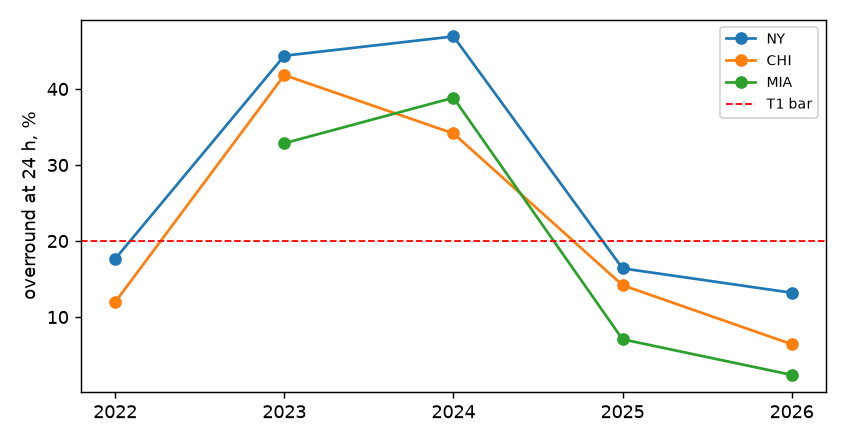
\includegraphics[width=0.75\linewidth]{figures/fig2_overround_by_year.png}
\caption{Markup (overround) of the replicating ladder at the 24 h ask, by city and year. Dashed line: the pre-registered 20\% limit.}
\label{fig:overround}
\end{figure}

The bigger issue is not the markup but what the price contains. The 24 h ask already knows tomorrow's forecast. A buyer who pays it gives up the weather swing and takes on a price swing of almost the same size. What is left to hedge is the forecast miss. Over all years, after paying the ask, the buyer's result is more variable than doing nothing ($\HElad = -0.32$). On 2025+ days it is 0.37, close to the 0.5 I wrote down as the expected value before the test (T1b, no pass bar). Two hours before the close, the price already knows the answer and $\HElad$ falls to 0.01. Figure~\ref{fig:hebyyear} shows both measures by year.

\begin{figure}[ht]
\centering
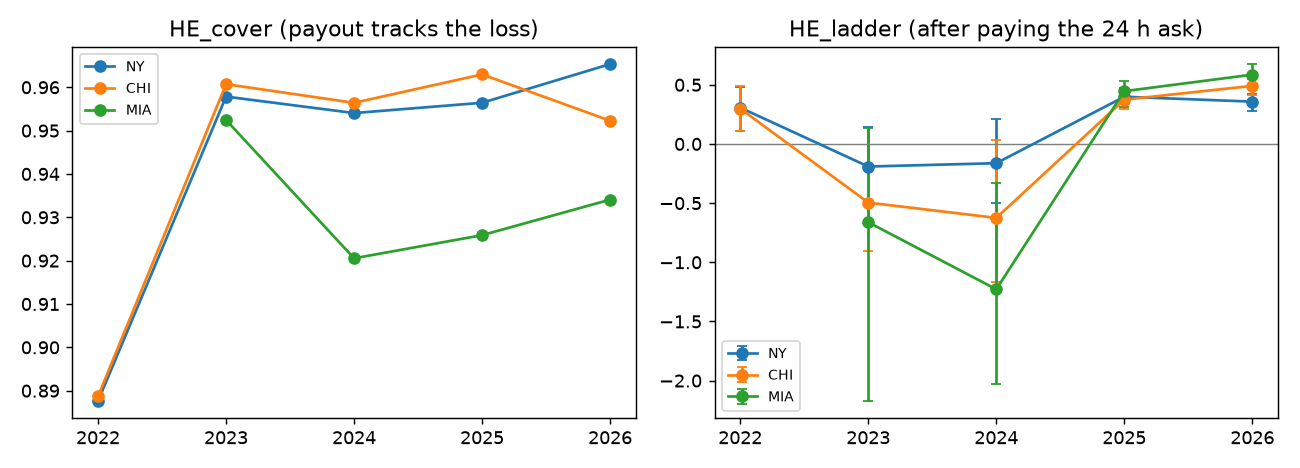
\includegraphics[width=\linewidth]{figures/fig1_he_by_year.png}
\caption{$\HEcov$ (left) and $\HElad$ at the 24 h ask (right) by city and year, strike rule A. Error bars: 95\% block bootstrap.}
\label{fig:hebyyear}
\end{figure}

This matters for how the product could work. A business that buys the ladder itself the day before gets the forecast miss, about 0.37 of the variance on the recent market, not 0.95. To give the business the 0.95, someone has to sell it a fixed-price policy in advance and then hedge day by day. That someone carries the forecast risk and needs capital for it (Section~\ref{sec:pool}).

Three other station results:
\begin{itemize}
\item \textbf{Thin ladders fail (T2).} Newark and Trenton ladders cost 241\% and 266\% more than they paid at 24 h, on 34 days each. A business near either city is better hedged with the New York ladder plus a residual.
\item \textbf{Liquidity (T4) fails on 2024 alone.} In Miami in 2024, at least one needed bracket had no offer on 13.7\% of days. In 2025 and 2026 the share was at most 0.3\%. From the one book snapshot, the thinnest needed bracket allows only 33, 54 and 55 units within 3 cents of slippage in New York, Chicago and Miami: a few dozen dollars per \degF{} per city-day.
\item \textbf{Fixed strike.} With the strike set in advance (rule B), the high fell outside the ladder's range on 3.1\% of days and the ladder bought nothing on 27\% of days; $\HElad$ was $-0.75$ over all years and $-0.20$ on 2025+ days.
\end{itemize}

\textbf{Rain (T3 passes).} Kalshi's daily ``any rain'' binary is a good forecast. Its 24 h Brier score is 0.106 against 0.247 for climatology, a gain of 0.141 [0.128, 0.152], far above the 0.02 bar. It costs \$1.20 per \$1 of payout at the 24 h ask with fees. For a wet-day exposure, $\HEcov$ is 0.83 and $\HElad$ is 0.27: the same forecast effect as for heat. In the KXRAIN series from July to September 2026, a trace of rain settled NO on all 26 trace days, so the cover counts a trace as dry to match. Under that rule (a labelled sensitivity run), $\HEcov$ is 0.76 and $\HElad$ 0.23.

\subsection{Away from the station: geography basis}
\label{sec:geo}

The residual tests use a 20-month test window (2025-01-01 to 2026-08-31: 608 days, or 86 Monday--Sunday weeks) and a 2024 training window used only to fit weights. The ``truth'' at each business location is a held-out airport weather station within 50 km of a settlement station: 37 temperature pairs and 26 rain pairs across five markets (New York, Newark, Trenton, Chicago Midway, Miami).

The station leg alone does well for heat and poorly for weekly rain (Table~\ref{tab:geo}, Figure~\ref{fig:geo}). For temperature, the pooled median HE at the held-out points is 0.81 [0.78, 0.84], against 0.95 at the station itself. For weekly rain it is 0.49 [0.38, 0.66], and in Miami only 0.13. Distance explains little: for heat, the worst points are sea-breeze sites, not the farthest ones. Rain falls off fast and unevenly, which fits convective summer storms.

\begin{table}[ht]
\centering
\small
\caption{Median HE of the station leg alone at held-out stations within 50 km, test window 2025-01 to 2026-08.}
\label{tab:geo}
\begin{tabular}{lcc}
\toprule
Market & Temperature (daily) & Rain (weekly) \\
\midrule
New York (Central Park) & 0.78 & 0.67 \\
Newark & 0.78 & 0.63 \\
Trenton & 0.87 & 0.47 \\
Chicago (Midway) & 0.84 & 0.69 \\
Miami & 0.67 & 0.13 \\
\midrule
Pooled median [95\% CI] & 0.81 [0.78, 0.84] & 0.49 [0.38, 0.66] \\
\bottomrule
\end{tabular}
\end{table}

\begin{figure}[ht]
\centering
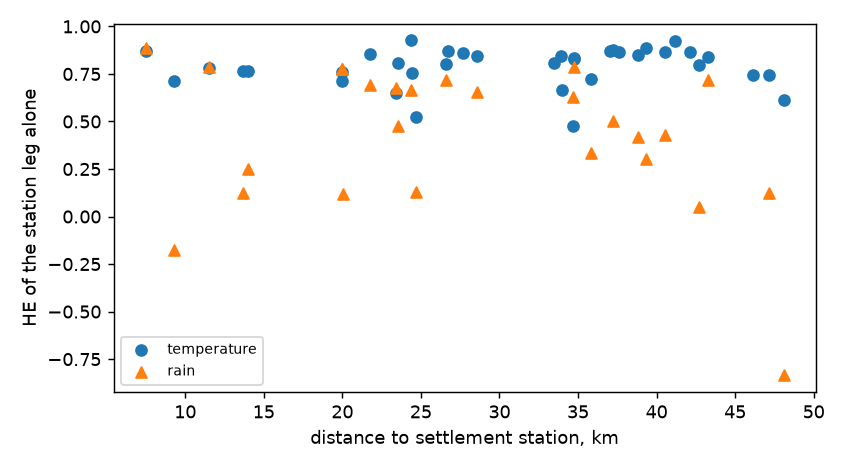
\includegraphics[width=0.7\linewidth]{figures/fig8_geography.png}
\caption{HE of the station leg alone at each held-out station, against distance to the settlement station.}
\label{fig:geo}
\end{figure}

One caution: these numbers use a strike that trails the recent mean. With Kalshi's own strike (set near the forecast) and the binned ladder as the station leg, the station-leg HE at nearby points falls to 0.36 (New York), 0.47 (Midway) and 0.27 (Miami). Payouts near the strike are sensitive to a 1--2\degF{} local difference.

\subsection{Residual contracts: rain passes, temperature does not}
\label{sec:residual}

I tested eight eligible residual designs plus continuity and exploratory variants. They fall into four groups: per-location grid cells (G1-P from PRISM, G1-N from nClimGrid), county averages (C1-N), regional factors that average a network of stations or grid cells around the settlement station (R-A, R-P, R-N), and nearby-station pairs (P-A, the nearest station; P-A-IDW, an inverse-distance average of the three nearest). In each case the residual pays the cover's payout at the local value minus the payout at the station value, so the business holds station leg plus residual. For G1-P, the residual is $H(P_{c(b)}) - H(P_{c(S)})$: the cover's payout on the PRISM cell containing the business minus its payout on the PRISM cell containing the station.

\begin{table}[ht]
\centering
\small
\caption{Residual bake-off, weekly rain totals, 26 pairs. $\dHE$ is the pooled median of per-pair gains over the station leg alone. The pooled median HE (0.81 for G1-P) and the median of the per-pair gains ($+0.229$) are different statistics, so 0.81 $-$ 0.49 need not equal 0.229.}
\label{tab:rain}
\footnotesize
\setlength{\tabcolsep}{3.5pt}
\begin{tabular}{llrrrrrl}
\toprule
Design & What it pays on & HE & $\dHE$ [95\% CI] & Pairs $>0$ & Mkts $>0$ & $\eta$ & Verdict \\
\midrule
D0 & Station only & 0.49 & --- & --- & --- & --- & baseline \\
G1-P & PRISM cell spread & 0.81 & $+0.229$ [0.119, 0.318] & 96\% & 5 & 0.76 & \textbf{survives} \\
R-A & Regional ASOS mean & 0.70 & $+0.110$ [0.055, 0.181] & 92\% & 5 & 0.79 & survives \\
G1-N & nClimGrid cell spread & 0.65 & $+0.091$ [0.043, 0.113] & 88\% & 5 & 1.73 & fails P1 \\
P-A-IDW & 3-station IDW & 0.75 & $+0.089$ [0.034, 0.137] & 85\% & 5 & 0.67 & fails P1 \\
R-P & Regional PRISM disc & 0.63 & $+0.073$ [0.014, 0.134] & 65\% & 4 & 0.73 & fails P1, P2 \\
R-N & Regional nClimGrid disc & 0.54 & $+0.029$ [0.011, 0.044] & 88\% & 5 & 2.47 & fails P1 \\
C1-N & County average & 0.62 & $+0.005$ [0.000, 0.034] & 75\% & 4 & 0.72 & fails P1 \\
P-A & Nearest station & 0.61 & $+0.001$ [0.000, 0.038] & 72\% & 3 & 0.42 & fails \\
\bottomrule
\end{tabular}
\end{table}

\textbf{Rain.} Table~\ref{tab:rain} and Figure~\ref{fig:bakeoff} show the weekly rain results. G1-P passed all four rules. On the 26 pairs, the pooled median HE rose from 0.49 with the station leg alone to 0.81 with the residual, and the median per-pair gain was $+0.229$ [0.119, 0.318]. The gain was positive at 25 of the 26 pairs and in all five markets (market medians $+0.21$ to $+0.24$). Its efficiency was $\eta = 0.76$: most of the variance the residual hands to the pool removes risk from the business. R-A also survived. G1-P won under the pre-registered rule (highest HE among survivors), ahead of R-A by 0.112 HE [0.032, 0.238].

Three things temper this result. First, G1-P's lead over the next-best design that failed, P-A-IDW, is only $+0.062$ [$-0.008$, 0.229], an interval that includes zero. Second, the gain is not uniform. In Miami the median HE with G1-P is still only 0.17, because the station leg starts so low there. Third, the gain is concentrated in the convective season (May--September $+0.357$) and is smaller in the most recent ten months ($+0.150$ for 2025-10 to 2026-08, a post-hoc sensitivity). I think the mechanism is that PRISM blends radar with dense volunteer rain gauges, while nClimGrid uses stations only and is heavily smoothed (its $\eta$ above 1 means its spread is too small).

There is also a gap between this result and the paper's main question. The weekly station leg here is the station's own weekly rainfall. Kalshi lists daily rain binaries and monthly rain ladders, not weekly totals, and the monthly ladders had no offer on 47--64\% of strikes at the start of the month. So the rain result shows that a two-leg index can track local weekly rain well; it does not show that the station leg of that index can be laid off on Kalshi today.

\begin{figure}[ht]
\centering
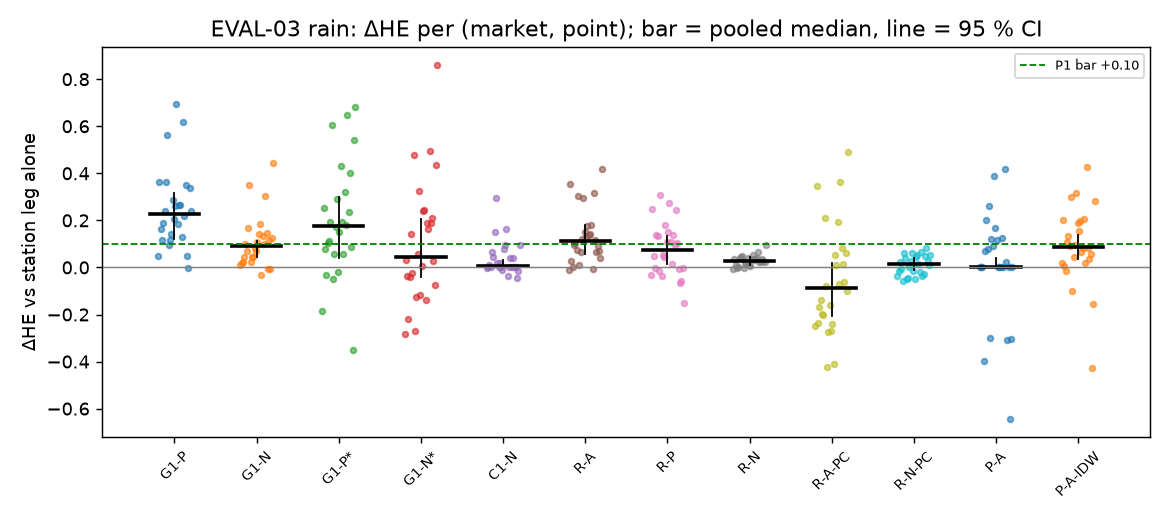
\includegraphics[width=\linewidth]{figures/bakeoff_dhe_rain.png}
\caption{Weekly rain: gain in HE over the station leg alone for each (market, held-out station) pair. Horizontal bar: pooled median; vertical line: 95\% CI; dashed line: the P1 bar of $+0.10$.}
\label{fig:bakeoff}
\end{figure}

\textbf{Temperature.} No design survived. The best, G1-P, raised HE from 0.81 to 0.87, a median gain of $+0.061$ [0.044, 0.075], with a gain at every pair. It failed P1 (gain below $+0.10$) and P3 ($\eta = 0.47$). P-A-IDW gained $+0.052$ and R-A $+0.033$. Two designs (C1-N and R-P) had a median gain at or below zero and were dropped. The reason is simple: within 50 km the station already carries most of the heat signal, so there is little left for a residual to remove. G1-P's temperature gain is also an upper bound, because every held-out station was an input to PRISM's temperature grid on the one day I could check. One sensitivity points the other way: with Kalshi's own forecast-centred strike, the basis is larger and the best residual gains are larger ($+0.161$ for G1-P, $+0.147$ for P-A-IDW). Under the pre-registered rule, heat cover is offered as the station leg alone, with any residual written as a custom quote.

\begin{figure}[ht]
\centering
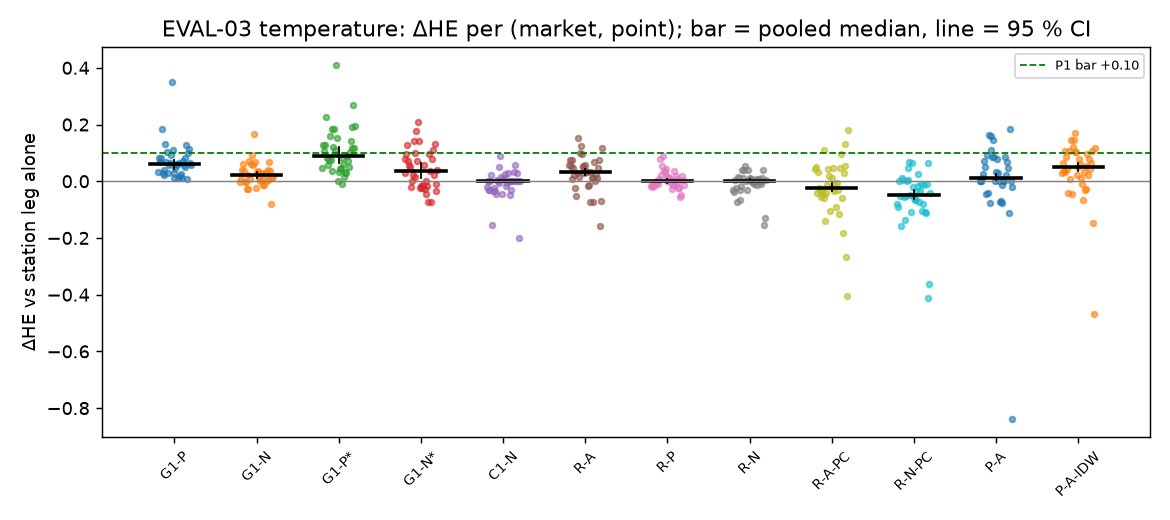
\includegraphics[width=\linewidth]{figures/bakeoff_dhe_temperature.png}
\caption{Daily temperature: gain in HE over the station leg alone for each (market, held-out station) pair. Same layout as Figure~\ref{fig:bakeoff}. No design reaches the $+0.10$ bar.}
\label{fig:bakeofft}
\end{figure}

Using frozen first-principal-component weights instead of equal weights in the regional designs made HE worse ($-0.055$ [$-0.080$, $-0.034$] for the ASOS network), so equal weights stay. That matches the finding that simple averages are hard to beat out of sample \citep{demiguel2009}.

\subsection{What a pool would carry}
\label{sec:pool}

If the business buys a fixed-price policy and the pool hedges, the pool carries the forecast risk and any flow it cannot pass on. I simulated this. The simulation built a business population around each settlement station from Census ZIP Business Patterns and published sector weather sensitivities (low-confidence priors), had 2\% of small establishments buy cover every warm-season day, cleared one uniform-price auction per station and day on real Kalshi-era days, and measured what the pool was left holding. Its residual leg is R-A, chosen before the residual bake-off ran; the capital for the station leg alone is reported next to it.

\textbf{Netting is small unless the priors are right.} Under the central sector priors, 40\% of gross hedge units cancel inside one station-day auction, and M1 passes with the minimum of 3 stations out of 5. If sector sensitivities are mostly common, which is what the best US daily evidence suggests, netting falls to 1.9\%. Rain nets to about zero (0.003), because nearly every sector loses on wet days.

\textbf{The pool cannot pass the flow to Kalshi.} Around Central Park, the pool is left with about 4,426 \$1/\degF{} units a day, against a Kalshi hedge capped at 5 units per city-day at today's depth. For a weekly rain book, Kalshi's daily rain markets could absorb about 704 contracts a day against roughly 205,019 needed. The pool is an insurer that uses Kalshi for pricing and some hedging, not a pass-through.

\begin{table}[ht]
\centering
\small
\caption{Pool capital from historical scenarios. $C_{30}$ = 30-day capital (the larger of ES99 and the worst historical 30-day loss, capped at full collateral). CPC = $C_{30}$ per \$ of 30-day pool notional; the pre-registered bar (M3) is 0.35. ``Climatology-priced'' rows price the cover before the forecast is known (added after the main run).}
\label{tab:capital}
\begin{tabular}{lrrrrr}
\toprule
Book & Seasons & $C_{30}$ & ES99 (30 d) & Junior ES95 & CPC \\
\midrule
Both legs (M3 headline) & 26 & \$412k & \$269k & \$206k & 0.126 \\
Station leg only & 64 & \$416k & \$278k & \$217k & 0.251 \\
Both legs, climatology-priced & 26 & \$577k & \$438k & \$337k & 0.177 \\
Station leg, climatology-priced & 64 & \$597k & \$438k & \$340k & 0.360 \\
\bottomrule
\end{tabular}
\end{table}

\textbf{Capital is affordable only with daily repricing.} The pool needs \$412k of 30-day capital, 0.126 per \$ of notional, so M3 passes (Table~\ref{tab:capital}). Three things make that headline look better than it is. The residual leg has a large notional and small risk, so it inflates the denominator; the station leg alone needs 0.25. The scenarios assume the cover is repriced each day from the forecast; if it is priced before the forecast is known, the station leg needs 0.36, over the bar. And the worst-window figure rests on 26 seasons (Figure~\ref{fig:capital}). The value-at-risk backtest (M5) was beaten once in 599 days against six expected; Kupiec's test \citep{kupiec1995} rejects ($p = 0.011$), in the conservative direction (the model holds too much).

\begin{figure}[ht]
\centering
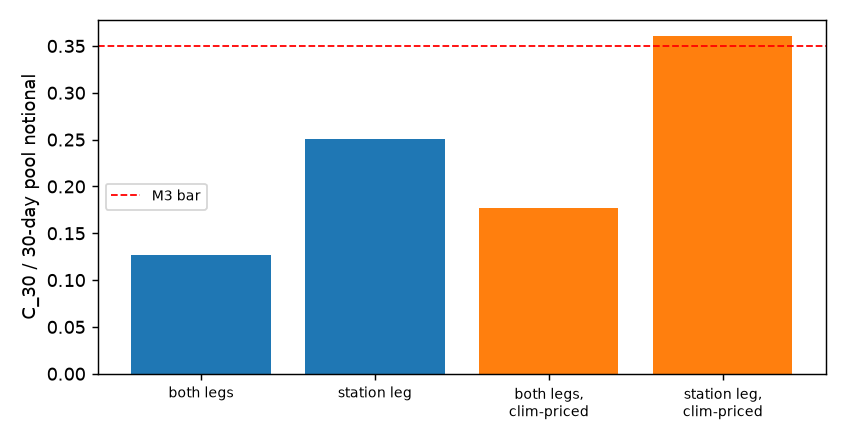
\includegraphics[width=0.7\linewidth]{figures/fig5_capital.png}
\caption{30-day pool capital per \$ of pool notional. Orange: cover priced before the forecast is known. Dashed line: the pre-registered 0.35 bar (M3).}
\label{fig:capital}
\end{figure}

\textbf{The first-loss layer fails its stress test.} In the design, a junior first-loss tranche (sized at the 30-day ES95, \$206k) takes losses before senior capital. A 30-day window understates a summer: the worst modelled season (2009) loses \$731k on the simulated book. With senior capital paid 20\% of the kept margin and a 10\% treasury cut, the junior layer's modelled return is $+43\%$ in the median season, $-144\%$ in a one-in-twenty season and $-332\%$ in the worst historical season. The pre-registered test (one-in-twenty return positive over three seasons) fails under every split rule, at $-190\%$ for the most favourable one. Under the split written in the design spec (senior paid 20\% of gross premium), the junior layer loses money even in the median modelled season ($-214\%$). The weekly rain book fails the same test ($-236\%$) and needs \$1,082k of 30-day capital. These numbers come from a block bootstrap of the capital scenario, not from observed seasons.

\textbf{House profits are not evidence.} The simulated house earned \$1,154 a day after hedging, but almost all of it came from the residual legs, mostly Central Park's, and that is a pricing artefact: Central Park reads cool against its neighbours and a long climatology underprices the residual. Priced on the trailing five years, the figure falls to \$384 a day. I do not lean on it.

\subsection{Can a business's weather sensitivity be learned?}
\label{sec:learn}

The design assumed a business could upload a year of daily sales, have its heat and rain sensitivity estimated, and buy a matching hedge. No public retail sales panel sits near a Kalshi city, so I tested this on stand-ins: bikeshare station trips (Citi Bike, Divvy), rail entries and taxi fares. These are demand proxies, not a shop's revenue, and bikeshare is far more weather-driven than a café, so these numbers are closer to an upper bound.

The learned hedge failed its main test (T2). Out of sample, the empirical-Bayes hedge removed 0.072 [0.056, 0.091] of daily revenue-surprise variance for Citi Bike stations and 0.053 [0.026, 0.077] for Divvy, against a bar of 0.20. Transit and taxi got about nothing. Almost all of the bike result came from the rain leg; the summer heat-only figure for Citi Bike was 0.001. Even a hedge fitted on the test year itself reached only 0.115, so the limit is the instrument (a heat call plus a wet-day binary), not the estimator. At real 24 h Kalshi prices with fees, the Citi Bike hedge kept $\HElad = 0.006$ and cost 32\% of payout, over the 25\% cap (T3 fails). The placebo test (P1) failed as written, and two rulings on this phase were made after the results; Section~\ref{sec:failures} gives the details. The honest summary is that rain sensitivity is real and learnable for bikeshare, and that whether a small shop's weather sensitivity can be learned and hedged is untested.

\section{Failed tests and changes after the freeze}
\label{sec:failures}

Most pre-registered tests in this project failed. Appendix~\ref{app:ledger} lists all 24 yes/no lines across the phases: 8 passed, 15 failed or triggered their pre-registered adverse branch, and 1 split between groups. The ones that matter most for the paper's question are:
\begin{itemize}
\item \textbf{T1 (station price).} The heat ladder's 24 h markup was 24.6\%, over the 20\% bar. This is the main negative result.
\item \textbf{T2 and T4.} Thin ladders cost more than three times what they paid out; liquidity failed in 2024.
\item \textbf{Temperature residual.} No design cleared the gain and efficiency bars.
\item \textbf{Junior layer.} The one-in-twenty three-season test failed for both the heat and the rain book.
\item \textbf{Learning.} T2, T3, T4 and the placebo P1 failed for every stand-in group.
\end{itemize}

Several changes were made after a freeze. I list the ones that touch a headline number:
\begin{itemize}
\item \textbf{The 2025+ pool} in Table~\ref{tab:station} was added after the full-sample numbers were seen. It is labelled post hoc everywhere and decides no test.
\item \textbf{Missing settled values.} For 205 Chicago, New York and Miami city-days (2025-10 to 2026-01) Kalshi's API returns no settled value; these were filled from the NWS climate report where it falls inside the bracket that settled YES (all 205 did). The strict frozen sample gives the same T1 and T4 verdicts.
\item \textbf{Missing PRISM cells.} At first, nine held-out points had no PRISM cell (the first pull kept only 40 km discs, and PRISM limits repeat downloads), so G1-P ran on 19 of 26 rain pairs and gained $+0.186$. A re-pull on 2026-10-02 added those cells. On all 26 pairs the gain is $+0.229$; the 19 earlier pairs did not change, and the winner did not change, but G1-P's lead over P-A-IDW shrank from a clear margin to an interval that includes zero. One temperature test day is still missing for the PRISM designs (an open data gap).
\item \textbf{Climatology-priced capital} (Table~\ref{tab:capital}) was added after the main capital run.
\item \textbf{Learning phase rulings.} The pre-registered placebo interval (DerSimonian--Laird, \citealp{dersimonian1986}) treated units as independent even though every unit in a city shares the same weather days; it called every placebo ``significant''. A joint day-block bootstrap, first run after a trial number, puts every placebo across zero and was adopted as the primary interval after the results. The pre-registered stop after Citi Bike's T1 failure was also overruled after the results. Both rulings are post hoc, and I report the results both ways.
\end{itemize}

\section{Limitations}
\label{sec:limits}

\begin{itemize}
\item \textbf{Prices come from hourly candles, not order books.} A missing hour is read as no change; the median staleness at 24 h is about an hour. Depth rests on one snapshot from 2026-09-29.
\item \textbf{The fee formula} is medium confidence and is applied to every year.
\item \textbf{Settlement source.} The tests measure the hedge against the NWS climate report. Kalshi's own series record for the New York daily high now names The Weather Company as the settlement source, while its help page still says NWS; the change seems to have been in place by mid-August 2026. On the 46 days per city settled under that source in my sample, the climate report disagreed with the settled value on 0\% (New York, Chicago) to 2.2\% (Miami) of days. I have not re-checked the station-leg numbers for dates after the change.
\item \textbf{Truth points are airports.} Real businesses sit in dense city centres, which may see more basis than any airport.
\item \textbf{Short windows.} The residual test window is 20 months; Trenton has two rain pairs. The capital tail rests on 26 joint seasons, and overlapping windows are not independent.
\item \textbf{PRISM revisions were not measured}, because PRISM keeps no prior versions. Any residual settled on PRISM needs the pool to archive the value it settles on. For nClimGrid, a preliminary value five days after the date differs from the final by at least half a degree on 64\% of cell-days.
\item \textbf{The pool is a simulation.} The business population, sector sensitivities and 2\% take-up are assumptions. The pool's residual leg in the capital runs (R-A) is not the residual the bake-off picked. The weekly rain book was sized but not built.
\item \textbf{No real sales.} The learning tests use public stand-ins. Whether a café's weather sensitivity is learnable and hedgeable needs a pilot with real sales data.
\item \textbf{No comparison with bespoke cover.} I had no quotes for custom weather contracts, so I cannot say whether this route is cheaper.
\item \textbf{Prototype only.} A prototype of the pool and auction was written as software and smart contracts, but nothing was deployed to any live network, no real money or real stablecoin was used, and no policy was sold. All pool results come from offline simulation.
\end{itemize}

\section{Conclusion}

Kalshi's daily weather contracts measure the right thing. At the settlement station, a ladder of them pays out almost exactly like a parametric heat cover, and the daily rain binary forecasts rain far better than climatology. As a hedge bought by the business itself, though, they keep only a small part of their value: the day-ahead price already contains the forecast, so a buyer keeps only the forecast miss, and over the full history the markup failed the pre-registered limit.

Two findings suggest where this could still work. A weekly rain residual built from PRISM grid cells closed much of the gap between the station and nearby locations, passing every pre-registered test; no temperature residual did. And the design that gives a business most of the station's 0.95 is a fixed-price policy written by a capitalised pool that hedges day by day. That pool's capital looks affordable only with daily repricing, its first-loss layer fails a one-in-twenty season, and it cannot pass its flow to Kalshi at today's depth.

The open questions are practical. Does the cheaper 2025--26 market hold up? Does the weekly rain residual hold in the next season, and can its station leg be hedged? And can a real small business's weather sensitivity be measured at all? The last one needs real sales data, not stand-ins.

\section*{Data and code}

All code, pre-registration files, results files and a map from every number in this paper to its source are in the project repository: \url{https://github.com/ehfuzzz/ceraunic-paper}. The file \texttt{paper/README.md} lists which script reproduces each table and figure.

\section*{Acknowledgments}

I am responsible for all errors. No external funding supported this work.

\bibliographystyle{plainnat}
\bibliography{refs}

\appendix

\section{Full ledger of pre-registered yes/no lines}
\label{app:ledger}

Each line was frozen before its phase produced a number. ``Adverse'' means the line fired the outcome the pre-registration named as the bad one. Freeze times are UTC on 2026-09-30.

\begin{small}
\begin{longtable}{p{2.6cm}p{6.0cm}p{3.6cm}p{2.2cm}}
\toprule
Phase / line & Rule & Result & Verdict \\
\midrule
\endhead
Station T1 (13:22) & Liquid ladders, 24 h, pooled: $\HEcov \ge 0.85$ and markup $\le 20\%$ & 0.95; 24.6\% & FAIL \\
Station T2 & Thin ladders fail if markup $> 100\%$ & EWR 241\%, TTN 266\% & FAIL \\
Station T3 & Rain Brier gain $\ge 0.02$ & 0.141 & PASS \\
Station T4 & No-offer $\le 10\%$ every city-year from 2024 & MIA 2024 13.7\% & FAIL \\
Station check & Reproduce an earlier New York study within 5\% & premium $-0.1\%$, payout 1.2\% & PASS \\
Residual heat (15:40) & P1--P4 all pass & best $+0.061$, $\eta$ 0.47 & FAIL \\
Residual rain (15:40) & P1--P4 all pass & G1-P $+0.229$, $\eta$ 0.76 & PASS \\
Residual Q2 & PC1 weights adopted only if HE higher by $\ge 0.03$, CI excl.\ 0 & $-0.055$ & FAIL (not adopted) \\
Pool M1 (13:26) & Netting $\ge 0.25$ at $\ge 3$ of 5 stations & 3 of 5 & PASS \\
Pool M2 & Null netting $< 0.10$ $\Rightarrow$ do not lead with netting & 0.019 & Adverse \\
Pool M3 & $C_{30}$ / notional $\le 0.35$ & 0.126 & PASS \\
Pool M4 & Payout-moving revisions $\le 2\%$ & 0.0\% & PASS \\
Pool M5 & Kupiec VaR99 not rejected at 5\% & 1 in 599, $p = 0.011$ & FAIL (conservative) \\
Junior (14:23) & 1-in-20 junior return positive over 3 seasons & $-190\%$ (best split) & FAIL \\
Rain book R1 (18:45) & Rain netting $\ge 0.25$ at $\ge 3$ of 5 & pooled 0.003 & FAIL \\
Rain book R2 & Two-leg $C_{30}$ / notional $\le 0.35$ & 0.166 & PASS \\
Rain book R3 & Two-leg / station $C_{30}$ $\le 1.25$ & 1.002 & PASS \\
Rain book R4 & Kalshi depth $\ge 0.5$ of need in $\ge 3$ of 5 & $\le 0.0092$ & FAIL \\
Rain book R5 & 1-in-20 junior return positive over 3 seasons & $-236\%$ (best split) & FAIL \\
Learning T1 (13:22) & Group heat and wet effects nonzero & Citi Bike heat not; Divvy both & Split \\
Learning T2 & Learned hedge HE $\ge 0.20$ & 0.072, 0.053 & FAIL \\
Learning T3 & HE after cost $> 0$ and cost $\le 25\%$ & 0.006, cost 32\% & FAIL \\
Learning T4 & Shrinkage beats own estimates by $\ge 0.02$ & 0.016 at $n = 180$ & FAIL \\
Learning P1 & Placebo insignificant and HE $\le 0.02$ & ``significant'' under DL & FAIL (as written) \\
\bottomrule
\end{longtable}
\end{small}

\end{document}
